% Options for packages loaded elsewhere
\PassOptionsToPackage{unicode}{hyperref}
\PassOptionsToPackage{hyphens}{url}
%
\documentclass[
]{article}
\usepackage{amsmath,amssymb}
\usepackage{lmodern}
\usepackage{iftex}
\ifPDFTeX
  \usepackage[T1]{fontenc}
  \usepackage[utf8]{inputenc}
  \usepackage{textcomp} % provide euro and other symbols
\else % if luatex or xetex
  \usepackage{unicode-math}
  \defaultfontfeatures{Scale=MatchLowercase}
  \defaultfontfeatures[\rmfamily]{Ligatures=TeX,Scale=1}
\fi
% Use upquote if available, for straight quotes in verbatim environments
\IfFileExists{upquote.sty}{\usepackage{upquote}}{}
\IfFileExists{microtype.sty}{% use microtype if available
  \usepackage[]{microtype}
  \UseMicrotypeSet[protrusion]{basicmath} % disable protrusion for tt fonts
}{}
\makeatletter
\@ifundefined{KOMAClassName}{% if non-KOMA class
  \IfFileExists{parskip.sty}{%
    \usepackage{parskip}
  }{% else
    \setlength{\parindent}{0pt}
    \setlength{\parskip}{6pt plus 2pt minus 1pt}}
}{% if KOMA class
  \KOMAoptions{parskip=half}}
\makeatother
\usepackage{xcolor}
\usepackage[margin=1in]{geometry}
\usepackage{color}
\usepackage{fancyvrb}
\newcommand{\VerbBar}{|}
\newcommand{\VERB}{\Verb[commandchars=\\\{\}]}
\DefineVerbatimEnvironment{Highlighting}{Verbatim}{commandchars=\\\{\}}
% Add ',fontsize=\small' for more characters per line
\usepackage{framed}
\definecolor{shadecolor}{RGB}{248,248,248}
\newenvironment{Shaded}{\begin{snugshade}}{\end{snugshade}}
\newcommand{\AlertTok}[1]{\textcolor[rgb]{0.94,0.16,0.16}{#1}}
\newcommand{\AnnotationTok}[1]{\textcolor[rgb]{0.56,0.35,0.01}{\textbf{\textit{#1}}}}
\newcommand{\AttributeTok}[1]{\textcolor[rgb]{0.77,0.63,0.00}{#1}}
\newcommand{\BaseNTok}[1]{\textcolor[rgb]{0.00,0.00,0.81}{#1}}
\newcommand{\BuiltInTok}[1]{#1}
\newcommand{\CharTok}[1]{\textcolor[rgb]{0.31,0.60,0.02}{#1}}
\newcommand{\CommentTok}[1]{\textcolor[rgb]{0.56,0.35,0.01}{\textit{#1}}}
\newcommand{\CommentVarTok}[1]{\textcolor[rgb]{0.56,0.35,0.01}{\textbf{\textit{#1}}}}
\newcommand{\ConstantTok}[1]{\textcolor[rgb]{0.00,0.00,0.00}{#1}}
\newcommand{\ControlFlowTok}[1]{\textcolor[rgb]{0.13,0.29,0.53}{\textbf{#1}}}
\newcommand{\DataTypeTok}[1]{\textcolor[rgb]{0.13,0.29,0.53}{#1}}
\newcommand{\DecValTok}[1]{\textcolor[rgb]{0.00,0.00,0.81}{#1}}
\newcommand{\DocumentationTok}[1]{\textcolor[rgb]{0.56,0.35,0.01}{\textbf{\textit{#1}}}}
\newcommand{\ErrorTok}[1]{\textcolor[rgb]{0.64,0.00,0.00}{\textbf{#1}}}
\newcommand{\ExtensionTok}[1]{#1}
\newcommand{\FloatTok}[1]{\textcolor[rgb]{0.00,0.00,0.81}{#1}}
\newcommand{\FunctionTok}[1]{\textcolor[rgb]{0.00,0.00,0.00}{#1}}
\newcommand{\ImportTok}[1]{#1}
\newcommand{\InformationTok}[1]{\textcolor[rgb]{0.56,0.35,0.01}{\textbf{\textit{#1}}}}
\newcommand{\KeywordTok}[1]{\textcolor[rgb]{0.13,0.29,0.53}{\textbf{#1}}}
\newcommand{\NormalTok}[1]{#1}
\newcommand{\OperatorTok}[1]{\textcolor[rgb]{0.81,0.36,0.00}{\textbf{#1}}}
\newcommand{\OtherTok}[1]{\textcolor[rgb]{0.56,0.35,0.01}{#1}}
\newcommand{\PreprocessorTok}[1]{\textcolor[rgb]{0.56,0.35,0.01}{\textit{#1}}}
\newcommand{\RegionMarkerTok}[1]{#1}
\newcommand{\SpecialCharTok}[1]{\textcolor[rgb]{0.00,0.00,0.00}{#1}}
\newcommand{\SpecialStringTok}[1]{\textcolor[rgb]{0.31,0.60,0.02}{#1}}
\newcommand{\StringTok}[1]{\textcolor[rgb]{0.31,0.60,0.02}{#1}}
\newcommand{\VariableTok}[1]{\textcolor[rgb]{0.00,0.00,0.00}{#1}}
\newcommand{\VerbatimStringTok}[1]{\textcolor[rgb]{0.31,0.60,0.02}{#1}}
\newcommand{\WarningTok}[1]{\textcolor[rgb]{0.56,0.35,0.01}{\textbf{\textit{#1}}}}
\usepackage{graphicx}
\makeatletter
\def\maxwidth{\ifdim\Gin@nat@width>\linewidth\linewidth\else\Gin@nat@width\fi}
\def\maxheight{\ifdim\Gin@nat@height>\textheight\textheight\else\Gin@nat@height\fi}
\makeatother
% Scale images if necessary, so that they will not overflow the page
% margins by default, and it is still possible to overwrite the defaults
% using explicit options in \includegraphics[width, height, ...]{}
\setkeys{Gin}{width=\maxwidth,height=\maxheight,keepaspectratio}
% Set default figure placement to htbp
\makeatletter
\def\fps@figure{htbp}
\makeatother
\setlength{\emergencystretch}{3em} % prevent overfull lines
\providecommand{\tightlist}{%
  \setlength{\itemsep}{0pt}\setlength{\parskip}{0pt}}
\setcounter{secnumdepth}{-\maxdimen} % remove section numbering
\usepackage{graphicx}
\usepackage{float}
\usepackage{booktabs}
\usepackage{longtable}
\usepackage{array}
\usepackage{multirow}
\usepackage{wrapfig}
\usepackage{float}
\usepackage{colortbl}
\usepackage{pdflscape}
\usepackage{tabu}
\usepackage{threeparttable}
\usepackage{threeparttablex}
\usepackage[normalem]{ulem}
\usepackage{makecell}
\usepackage{xcolor}
\ifLuaTeX
  \usepackage{selnolig}  % disable illegal ligatures
\fi
\IfFileExists{bookmark.sty}{\usepackage{bookmark}}{\usepackage{hyperref}}
\IfFileExists{xurl.sty}{\usepackage{xurl}}{} % add URL line breaks if available
\urlstyle{same} % disable monospaced font for URLs
\hypersetup{
  pdftitle={Mandatory Assignment 1 AEF},
  pdfauthor={ncx951 \& dsc579},
  hidelinks,
  pdfcreator={LaTeX via pandoc}}

\title{Mandatory Assignment 1 AEF}
\author{ncx951 \& dsc579}
\date{2023-04-03}

\begin{document}
\maketitle

\hypertarget{excercise-1}{%
\section{Excercise 1}\label{excercise-1}}

\begin{Shaded}
\begin{Highlighting}[]
\CommentTok{\# Load in the dataset}
\NormalTok{tidy\_finance }\OtherTok{\textless{}{-}} \FunctionTok{dbConnect}\NormalTok{(}
  \FunctionTok{SQLite}\NormalTok{(),}
  \StringTok{"tidy\_finance\_ML.sqlite"}\NormalTok{,}
  \AttributeTok{extended\_types =} \ConstantTok{TRUE}
\NormalTok{)}
\NormalTok{stock\_characteristics\_monthly }\OtherTok{\textless{}{-}} \FunctionTok{tbl}\NormalTok{(tidy\_finance, }\StringTok{"stock\_characteristics\_monthly"}\NormalTok{) }\SpecialCharTok{|\textgreater{}} \FunctionTok{collect}\NormalTok{()}

\CommentTok{\# Renaming column names according to the names from the Gu et al paper}

\FunctionTok{colnames}\NormalTok{(stock\_characteristics\_monthly) }\OtherTok{\textless{}{-}} \FunctionTok{c}\NormalTok{(}\StringTok{"permno"}\NormalTok{, }\StringTok{"month"}\NormalTok{, }\StringTok{"ret\_excess"}\NormalTok{, }\StringTok{"mktcap\_lag"}\NormalTok{, }\StringTok{"sic2"}\NormalTok{, }
                                             \StringTok{"m\_bm"}\NormalTok{, }\StringTok{"m\_ntis"}\NormalTok{, }\StringTok{"m\_tbl"}\NormalTok{, }\StringTok{"m\_dfy"}\NormalTok{,}
                                             \StringTok{"c\_mom1m"}\NormalTok{, }\StringTok{"c\_mom12m"}\NormalTok{, }\StringTok{"c\_chmom"}\NormalTok{, }\StringTok{"c\_maxret"}\NormalTok{, }\StringTok{"c\_mvel1"}\NormalTok{)}


\CommentTok{\# Filtering out characteristics and only include data from 2005{-}01{-}01}
\NormalTok{stock\_characteristics\_monthly }\OtherTok{\textless{}{-}}\NormalTok{ stock\_characteristics\_monthly }\SpecialCharTok{|\textgreater{}}
               \FunctionTok{select}\NormalTok{(permno, month, ret\_excess, mktcap\_lag, sic2, }
\NormalTok{                      m\_bm, m\_ntis, m\_tbl, m\_dfy, }
\NormalTok{                      c\_mom1m, c\_mom12m, c\_chmom, c\_maxret, c\_mvel1) }\SpecialCharTok{|\textgreater{}}     
               \FunctionTok{filter}\NormalTok{(month }\SpecialCharTok{\textgreater{}=} \StringTok{"2005{-}01{-}01"}\NormalTok{) }\SpecialCharTok{|\textgreater{}}
               \FunctionTok{drop\_na}\NormalTok{()}

\CommentTok{\# Turn sic2 into a factor instead of numerical value}
\NormalTok{stock\_characteristics\_monthly}\SpecialCharTok{$}\NormalTok{sic2 }\OtherTok{\textless{}{-}} \FunctionTok{as.factor}\NormalTok{(stock\_characteristics\_monthly}\SpecialCharTok{$}\NormalTok{sic2)}

\CommentTok{\# Convert month column to Date format}
\NormalTok{stock\_characteristics\_monthly}\SpecialCharTok{$}\NormalTok{month }\OtherTok{\textless{}{-}} \FunctionTok{as.Date}\NormalTok{(stock\_characteristics\_monthly}\SpecialCharTok{$}\NormalTok{month)}

\FunctionTok{dbDisconnect}\NormalTok{(tidy\_finance)}
\FunctionTok{remove}\NormalTok{(tidy\_finance)}
\end{Highlighting}
\end{Shaded}

The dataset includes observations from January 1st 2005.

We make summary statistics below

\begin{Shaded}
\begin{Highlighting}[]
\CommentTok{\# Counting how many firms (permno) thats in each industry (sic2) for each month}
\NormalTok{no\_industry }\OtherTok{\textless{}{-}} \FunctionTok{select}\NormalTok{(stock\_characteristics\_monthly, permno, month, sic2) }\SpecialCharTok{|\textgreater{}}
                \FunctionTok{group\_by}\NormalTok{(month, sic2) }\SpecialCharTok{|\textgreater{}}
                \FunctionTok{summarise}\NormalTok{(}\AttributeTok{n =} \FunctionTok{n}\NormalTok{())}

\CommentTok{\# Creates a stacked barplot}
\FunctionTok{ggplot}\NormalTok{(no\_industry, }\FunctionTok{aes}\NormalTok{(}\AttributeTok{fill=}\NormalTok{sic2, }\AttributeTok{y=}\NormalTok{n, }\AttributeTok{x=}\NormalTok{month)) }\SpecialCharTok{+}
  \FunctionTok{geom\_bar}\NormalTok{(}\AttributeTok{position =} \StringTok{"stack"}\NormalTok{, }\AttributeTok{stat =} \StringTok{"identity"}\NormalTok{) }\SpecialCharTok{+}
  \FunctionTok{ggtitle}\NormalTok{(}\StringTok{"Number of unique firms (permno) in each industry classification (sic2) for each month"}\NormalTok{) }\SpecialCharTok{+} 
  \FunctionTok{xlab}\NormalTok{(}\StringTok{"Time"}\NormalTok{) }\SpecialCharTok{+} 
  \FunctionTok{ylab}\NormalTok{(}\StringTok{"No. firms"}\NormalTok{) }\SpecialCharTok{+}
  \FunctionTok{scale\_fill\_discrete}\NormalTok{(}\AttributeTok{name =} \StringTok{"Industry classifications (sic2)"}\NormalTok{)}
\end{Highlighting}
\end{Shaded}

\begin{center}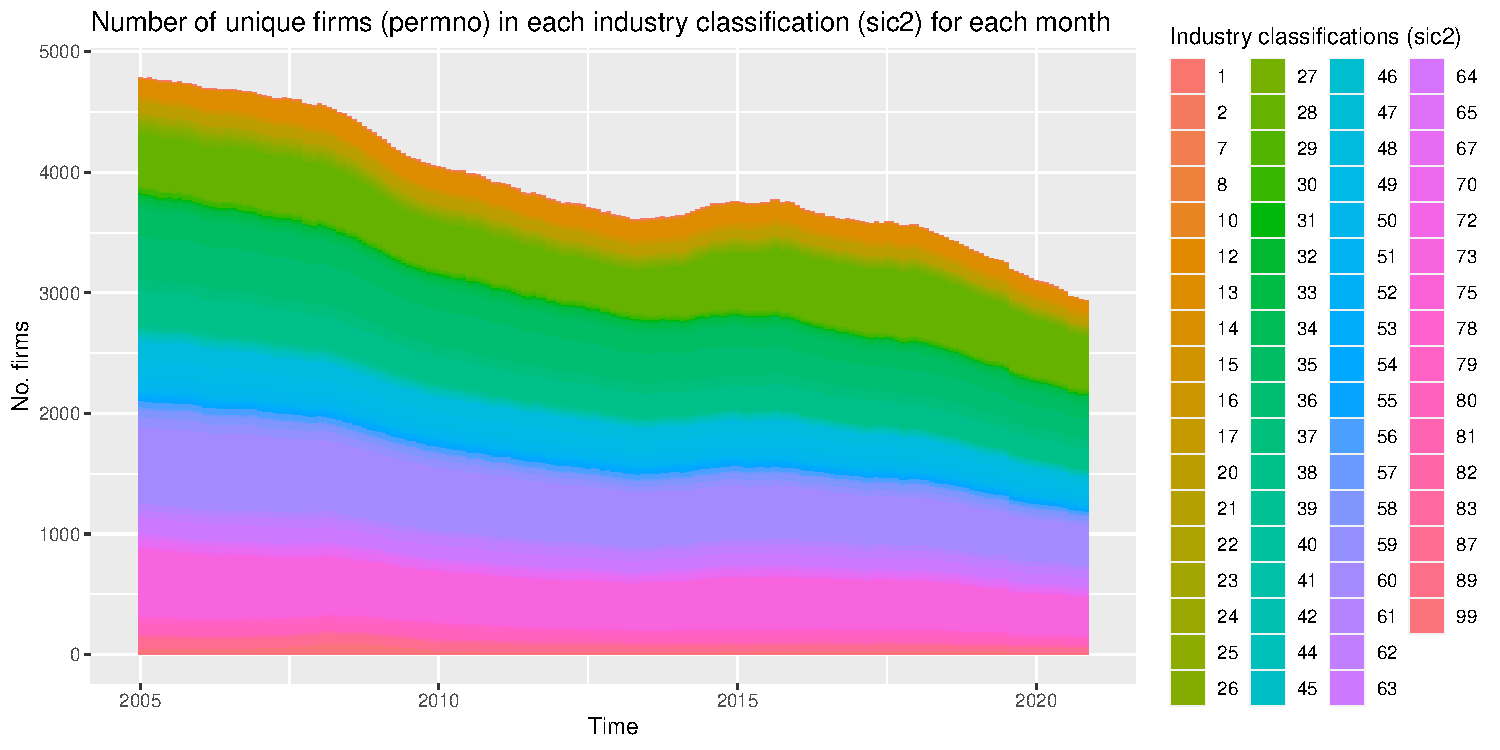
\includegraphics{figure/graphics-unnamed-chunk-3-1} \end{center}

Summary table

\begin{Shaded}
\begin{Highlighting}[]
\NormalTok{stock\_characteristics\_monthly\_summary }\OtherTok{\textless{}{-}}\NormalTok{ stock\_characteristics\_monthly }\SpecialCharTok{|\textgreater{}}
  \FunctionTok{select}\NormalTok{(}\SpecialCharTok{{-}}\NormalTok{permno, }\SpecialCharTok{{-}}\NormalTok{month, }\SpecialCharTok{{-}}\NormalTok{sic2) }\SpecialCharTok{|\textgreater{}}
  \FunctionTok{pivot\_longer}\NormalTok{(}\AttributeTok{cols =} \FunctionTok{everything}\NormalTok{(), }\AttributeTok{names\_to =} \StringTok{"Variables"}\NormalTok{, }\AttributeTok{values\_to =} \StringTok{"Value"}\NormalTok{) }\SpecialCharTok{|\textgreater{}}
  \FunctionTok{group\_by}\NormalTok{(Variables) }\SpecialCharTok{|\textgreater{}}
  \FunctionTok{summarize\_all}\NormalTok{(}\FunctionTok{list}\NormalTok{(}\AttributeTok{mean =}\NormalTok{ mean, }
                     \AttributeTok{sd =}\NormalTok{ sd,}
                     \AttributeTok{min =}\NormalTok{ min,}
                     \AttributeTok{median =}\NormalTok{ median,}
                     \AttributeTok{max =}\NormalTok{ max)) }\SpecialCharTok{|\textgreater{}}
\NormalTok{  knitr}\SpecialCharTok{::}\FunctionTok{kable}\NormalTok{(}\AttributeTok{booktabs =} \ConstantTok{TRUE}\NormalTok{, }\AttributeTok{digits =} \DecValTok{2}\NormalTok{, }\AttributeTok{caption =} \StringTok{"Summary statistics of the predictors"}\NormalTok{) }\SpecialCharTok{|\textgreater{}} 
  \FunctionTok{kable\_paper}\NormalTok{(}\StringTok{"hover"}\NormalTok{, }\AttributeTok{full\_width =}\NormalTok{ T) }\SpecialCharTok{|\textgreater{}}  
  \FunctionTok{group\_rows}\NormalTok{(}\StringTok{"Stock Characteristics"}\NormalTok{, }\DecValTok{1}\NormalTok{, }\DecValTok{5}\NormalTok{) }\SpecialCharTok{|\textgreater{}} 
  \FunctionTok{group\_rows}\NormalTok{(}\StringTok{"Macro Characteristics"}\NormalTok{, }\DecValTok{6}\NormalTok{, }\DecValTok{9}\NormalTok{) }\SpecialCharTok{|\textgreater{}} 
  \FunctionTok{group\_rows}\NormalTok{(}\StringTok{"Initial Variables"}\NormalTok{, }\DecValTok{10}\NormalTok{, }\DecValTok{11}\NormalTok{)}

\NormalTok{stock\_characteristics\_monthly\_summary}
\end{Highlighting}
\end{Shaded}

\begin{table}

\caption{\label{tab:unnamed-chunk-4}Summary statistics of the predictors}
\centering
\begin{tabu} to \linewidth {>{\raggedright}X>{\raggedleft}X>{\raggedleft}X>{\raggedleft}X>{\raggedleft}X>{\raggedleft}X}
\toprule
Variables & mean & sd & min & median & max\\
\midrule
\addlinespace[0.3em]
\multicolumn{6}{l}{\textbf{Stock Characteristics}}\\
\hspace{1em}c\_chmom & -0.01 & 0.02 & -0.06 & -0.01 & 0.03\\
\hspace{1em}c\_maxret & 0.01 & 0.02 & 0.00 & 0.00 & 0.05\\
\hspace{1em}c\_mom12m & 0.30 & 0.05 & 0.22 & 0.31 & 0.44\\
\hspace{1em}c\_mom1m & 0.00 & 0.01 & 0.00 & 0.00 & 0.07\\
\hspace{1em}c\_mvel1 & 0.03 & 0.01 & 0.01 & 0.03 & 0.05\\
\addlinespace[0.3em]
\multicolumn{6}{l}{\textbf{Macro Characteristics}}\\
\hspace{1em}m\_bm & -3.92 & 0.14 & -4.13 & -3.94 & -3.28\\
\hspace{1em}m\_dfy & -0.83 & 0.51 & -1.24 & -0.97 & 1.38\\
\hspace{1em}m\_ntis & -3.91 & 0.13 & -4.12 & -3.93 & -3.29\\
\hspace{1em}m\_tbl & -3.09 & 0.41 & -4.84 & -2.99 & -2.57\\
\addlinespace[0.3em]
\multicolumn{6}{l}{\textbf{Initial Variables}}\\
\hspace{1em}mktcap\_lag & 4908.72 & 24797.13 & 0.09 & 451.96 & 2206911.13\\
\hspace{1em}ret\_excess & 0.01 & 0.18 & -1.00 & 0.00 & 19.88\\
\bottomrule
\end{tabu}
\end{table}

We now make the recipe

\begin{Shaded}
\begin{Highlighting}[]
\NormalTok{rec }\OtherTok{\textless{}{-}} \FunctionTok{recipe}\NormalTok{(ret\_excess }\SpecialCharTok{\textasciitilde{}}\NormalTok{ ., }\AttributeTok{data =}\NormalTok{ stock\_characteristics\_monthly) }\SpecialCharTok{|\textgreater{}}
  \FunctionTok{step\_rm}\NormalTok{(permno}\SpecialCharTok{:}\NormalTok{month) }\SpecialCharTok{|\textgreater{}}
  \FunctionTok{step\_interact}\NormalTok{(}\AttributeTok{terms =} \SpecialCharTok{\textasciitilde{}}\FunctionTok{contains}\NormalTok{(}\StringTok{"c\_"}\NormalTok{)}\SpecialCharTok{:}\FunctionTok{contains}\NormalTok{(}\StringTok{"m\_"}\NormalTok{)) }\SpecialCharTok{|\textgreater{}}
  \FunctionTok{step\_dummy}\NormalTok{(sic2, }\AttributeTok{one\_hot =} \ConstantTok{TRUE}\NormalTok{) }\SpecialCharTok{|\textgreater{}}
  \FunctionTok{step\_normalize}\NormalTok{(}\FunctionTok{all\_predictors}\NormalTok{()) }\SpecialCharTok{|\textgreater{}}
  \FunctionTok{step\_center}\NormalTok{(ret, }\AttributeTok{skip =} \ConstantTok{TRUE}\NormalTok{)}
\end{Highlighting}
\end{Shaded}

\hypertarget{excercise-2}{%
\section{Excercise 2}\label{excercise-2}}

Gu et al.~(2020) describe an asset's excess return as an additive
prediction error model the following way:

\[r_{i,t+1} = E_t(r_{i,t+1}) + \varepsilon_{i,t+1} \quad \text{where} \quad E_t(r_{i,t+1}) = g(z_{i,t})\]
Where \(g(z_{i,t})\) is a function of the \(P\)-dimensional vector
\(z_{i,t}\) of predictor variables.

As stated in the paper this would be considered a very flexible model,
however it imposes some important restrictions. First the \(g(\cdot)\)
function depends neither on the individual stock or time period. It thus
leverages of the information from the entire dataset. The functional
form thus doesn't adjust by time period or for specific stocks. For
example one variable could have a larger explanatory power in the
beginning of the time period but much lesser towards the end. The effect
from the predictor would still remain constant, and could also relate to
overfitting the model. The model also assumes that the prediction error
\(\varepsilon_{i,t+1}\) is additive and independent of the predictor
variables, which may not hold in reality.

\hypertarget{excercise-3}{%
\section{Excercise 3}\label{excercise-3}}

Making the train-validation-test split with 20\% of the last
observations as test data and make 20\% of the train data into
validation.

\begin{Shaded}
\begin{Highlighting}[]
\NormalTok{test\_data }\OtherTok{\textless{}{-}}\NormalTok{ stock\_characteristics\_monthly }\SpecialCharTok{|\textgreater{}}
  \FunctionTok{filter}\NormalTok{(month }\SpecialCharTok{\textgreater{}} \StringTok{"2017{-}02{-}01"}\NormalTok{) }
  

\NormalTok{validation\_data }\OtherTok{\textless{}{-}}\NormalTok{ stock\_characteristics\_monthly }\SpecialCharTok{|\textgreater{}}
  \FunctionTok{filter}\NormalTok{(month }\SpecialCharTok{\textgreater{}=} \StringTok{"2014{-}07{-}01"}\NormalTok{, month }\SpecialCharTok{\textless{}=}\StringTok{"2017{-}02{-}01"}\NormalTok{)}

\NormalTok{train\_data }\OtherTok{\textless{}{-}}\NormalTok{ stock\_characteristics\_monthly }\SpecialCharTok{|\textgreater{}}
  \FunctionTok{filter}\NormalTok{(month }\SpecialCharTok{\textless{}} \StringTok{"2014{-}07{-}01"}\NormalTok{)}
\end{Highlighting}
\end{Shaded}

\hypertarget{excercise-4}{%
\section{Excercise 4}\label{excercise-4}}

Neural Network

\begin{Shaded}
\begin{Highlighting}[]
\NormalTok{lambda }\OtherTok{\textless{}{-}} \FloatTok{0.0001}
\NormalTok{dropout\_rate }\OtherTok{\textless{}{-}} \FloatTok{0.05}

\NormalTok{NN\_model }\OtherTok{\textless{}{-}} \FunctionTok{keras\_model\_sequential}\NormalTok{() }\SpecialCharTok{|\textgreater{}}
    \FunctionTok{layer\_dense}\NormalTok{(}\AttributeTok{units =} \DecValTok{10}\NormalTok{, }\AttributeTok{activation =} \StringTok{"sigmoid"}\NormalTok{, }\AttributeTok{input\_shape =} \DecValTok{13}\NormalTok{, }\AttributeTok{kernel\_regularizer =} \FunctionTok{regularizer\_l2}\NormalTok{(lambda)) }\SpecialCharTok{|\textgreater{}}
    \FunctionTok{layer\_dropout}\NormalTok{(}\AttributeTok{rate=}\NormalTok{dropout\_rate) }\SpecialCharTok{|\textgreater{}}
    \FunctionTok{layer\_dense}\NormalTok{(}\AttributeTok{units =} \DecValTok{10}\NormalTok{, }\AttributeTok{activation =} \StringTok{"sigmoid"}\NormalTok{, }\AttributeTok{kernel\_regularizer =} \FunctionTok{regularizer\_l2}\NormalTok{(lambda)) }\SpecialCharTok{|\textgreater{}}
    \FunctionTok{layer\_dropout}\NormalTok{(}\AttributeTok{rate=}\NormalTok{dropout\_rate) }\SpecialCharTok{|\textgreater{}}
    \FunctionTok{layer\_dense}\NormalTok{(}\AttributeTok{units =} \DecValTok{10}\NormalTok{, }\AttributeTok{activation =} \StringTok{"sigmoid"}\NormalTok{, }\AttributeTok{kernel\_regularizer =} \FunctionTok{regularizer\_l2}\NormalTok{(lambda)) }\SpecialCharTok{|\textgreater{}}
    \FunctionTok{layer\_dropout}\NormalTok{(}\AttributeTok{rate=}\NormalTok{dropout\_rate) }\SpecialCharTok{|\textgreater{}}
    \FunctionTok{layer\_dense}\NormalTok{(}\AttributeTok{units =} \DecValTok{1}\NormalTok{, }\AttributeTok{activation =} \StringTok{"linear"}\NormalTok{) }\SpecialCharTok{|\textgreater{}}

  \FunctionTok{compile}\NormalTok{(}
    \AttributeTok{loss =} \StringTok{\textquotesingle{}mse\textquotesingle{}}\NormalTok{,}
    \AttributeTok{optimizer =} \FunctionTok{optimizer\_rmsprop}\NormalTok{(}\AttributeTok{learning\_rate=}\FloatTok{0.001}\NormalTok{, }\AttributeTok{rho=}\FloatTok{0.9}\NormalTok{)    }
\NormalTok{)}
\end{Highlighting}
\end{Shaded}


\end{document}
